\documentclass{echw}

\title{Assignment A10.4\\Complex Numbers}
\author{Eytan Chong}
\date{2024-08-02}

\begin{document}
    \problem{}
        On a single Argand diagram, sketch the following loci.
        \begin{enumerate}
            \item $\abs{z - 2i} = 4$.
            \item $\arg{\dfrac{7}{z + 2}} = -\dfrac\pi4$.
        \end{enumerate}

        Hence, or otherwise, find the exact value of $z$ satisfying both equations in part (a) and (b).

    \solution
        Note that $\arg{\dfrac{7}{z + 2}} = -\dfrac\pi4 \implies \arg{z - (-2)} = \dfrac\pi4$.
        \begin{center}
            \begin{tikzpicture}[trim axis left, trim axis right]
                \begin{axis}[
                    domain = 0:10,
                    samples = 101,
                    axis y line=middle,
                    axis x line=middle,
                    xtick = {-2},
                    ytick = {6, 2, -2},
                    xmax=5.75,
                    xmin=-5.75,
                    ymin=-3,
                    ymax=7,
                    xlabel = {$\Re$},
                    ylabel = {$\Im$},
                    legend cell align={left},
                    legend pos=outer north east,
                    after end axis/.code={
                        \path (axis cs:0,0) 
                            node [anchor=north east] {$O$};
                        }
                    ]
        
                    \coordinate (R) at (10,0);
                    \coordinate (Z) at (-2, 0);
                    \coordinate[label=below right:$C$] (C) at (0, 2);
                    \coordinate (O) at (0, 0);

                    \draw[plotRed] (C) circle[radius=4];
            
                    \draw (O) -- (Z);

                    \draw[plotBlue] (Z) -- (6, 8);
            
                    \fill (C) circle[radius=2.5pt];
                    \draw (Z) circle[radius=2.5pt];

                    \draw pic [draw, angle radius=10mm, "$\frac{\pi}4$"] {angle = R--Z--C};
                    
                    \draw[dotted] (C) -- (4, 2);
                    \node[above] at (2, 2) {4};

                    \addlegendimage{plotRed};
                    \addlegendentry{locus of $\abs{z - 2i} = 4$};

                    \addlegendimage{plotBlue};
                    \addlegendentry{locus of $\arg{\frac{7}{z + 2}} = -\frac\pi4$};
                \end{axis}
            \end{tikzpicture}
        \end{center}
        \begin{align*}
            z &= 2i + \bp{\cos \dfrac\pi4 + i\sin\dfrac\pi4}\\
            &= 2i + \dfrac{\sqrt2}2 + i\dfrac{\sqrt2}2\\
            &= \boxed{\dfrac{\sqrt2}2 + \bp{2 + \dfrac{\sqrt2}2} i}
        \end{align*}

    \problem{}
        Given that $\abs{z - 2i} \leq 4$, illustrate the locus of the point representing the complex number $z$ in an Argand diagram.

        Hence, find the greatest and least possible value of $\abs{z - 3 + 4i}$, given that $\abs{z - 2i} \leq 4$.

    \solution
        \begin{center}
            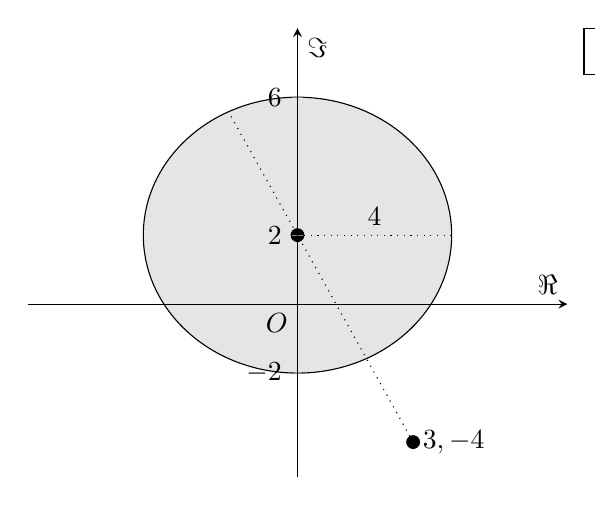
\begin{tikzpicture}[trim axis left, trim axis right]
                \begin{axis}[
                    axis on top,
                    domain = 0:10,
                    samples = 101,
                    axis y line=middle,
                    axis x line=middle,
                    xtick = \empty,
                    ytick = {6, 2, -2},
                    xmax=7,
                    xmin=-7,
                    ymin=-5,
                    ymax=8,
                    xlabel = {$\Re$},
                    ylabel = {$\Im$},
                    legend cell align={left},
                    legend pos=outer north east,
                    after end axis/.code={
                        \path (axis cs:0,0) 
                            node [anchor=north east] {$O$};
                        }
                    ]
        
                    \coordinate (R) at (10,0);
                    \coordinate[label=right:$\bp{3, -4}$] (Z) at (3, -4);
                    \coordinate[label=below right:$C$] (C) at (0, 2);
                    \coordinate (O) at (0, 0);

                    \fill[black!10] (C) circle[radius=4];
                    \draw (C) circle[radius=4];
            
                    \draw[dotted] (Z) -- (-1.7889, 5.5771);
            
                    \fill (Z) circle[radius=2.5pt];
                    \fill (C) circle[radius=2.5pt];
                    
                    \draw[dotted] (C) -- (4, 2);
                    \node[above] at (2, 2) {4};

                    \addlegendimage{line legend, black!10, line width=5pt}
                    \addlegendentry{required locus};
                \end{axis}
            \end{tikzpicture}
        \end{center}
        Note that $\abs{z - 3 + 4i} = \abs{z - (3 - 4i)}$ represents the distance between $z$ and the point $(3, -4)$.

        By Pythagoras' Theorem, the distance between the centre of the circle $(0, 2)$ and $(3, -4)$ is $\sqrt{(0-3)^2 + (2  + 4)^2} = 3\sqrt5$. Hence, $\max \abs{z - 3 + 4i} = 3\sqrt5 + 4$, while $\min \abs{z - 3 + 4i} = 3\sqrt5 - 4$.

        \boxt{$\max \abs{z - 3 + 4i} = 3\sqrt5 + 4$, $\min \abs{z - 3 + 4i} = 3\sqrt5 - 4$}

    \problem{}
        The point $A$ on an Argand diagram represents the fixed complex number $a$, where $0 < \arg a < \dfrac\pi2$. The complex numbers $z$ and $w$ are such that $\abs{z - 2ia} = \abs{a}$ and $\abs{w} = \abs{w + ia}$.

        Sketch, on a single diagram, the loci of the point representing $z$ and $w$.
        
        Find
        \begin{enumerate}
            \item the minimum value of $\abs{z - w}$ in terms of $\abs{a}$,
            \item the range of values of $\arg \dfrac1z$ in terms of $\arg a$.
        \end{enumerate}

    \solution
        Note that $\abs{w} = \abs{w + ia} \implies \abs{w - 0} = \abs{w - (-ia)}$.
        \begin{center}
            \begin{tikzpicture}[trim axis left, trim axis right]
                \begin{axis}[
                    domain = -10:0,
                    samples = 101,
                    axis y line=middle,
                    axis x line=middle,
                    xtick = \empty,
                    ytick = \empty,
                    xmax=2.5,
                    xmin=-3.5,
                    ymin=-1.7,
                    ymax=3.5,
                    xlabel = {$\Re$},
                    ylabel = {$\Im$},
                    legend cell align={left},
                    legend pos=outer north east,
                    after end axis/.code={
                        \path (axis cs:0,0) 
                            node [anchor=north east] {$O$};
                        }
                    ]
        
                    \coordinate (R) at (10,0);
                    \coordinate[label=above:$A(a)$] (A) at (1, 1);
                    \coordinate[label=above:$C(2ia)$] (C) at (-2, 2);
                    \coordinate[label=below:$B(-ia)$] (B) at (1, -1);
                    \coordinate (O) at (0, 0);
                    \coordinate (B') at (0.5, -0.5);
                    \coordinate (B'') at (1, 0);
                    \coordinate[label=right:$D$] (D) at (-0.633975, 2.36603);
                    \coordinate[label=below left:$E$] (E) at (-2.36603, 0.633975);
            
                    \draw[dotted] (O) -- (A);
                    \draw[dotted] (B) -- (C);

                    \draw[dotted] (C) -- (-2-1.414, 2);
                    \node[below] at (-2-0.707, 2) {$\abs{a}$};

                    \draw[plotRed] (C) circle[radius=1.414];

                    \addplot[plotBlue, domain=-2:3] {x - 1};

                    \addplot[domain=0.15:0.35] {x - 0.5};
                    \addplot[domain=0.65:0.85] {x - 1.5};
            
                    \fill (A) circle[radius=2.5pt];
                    \fill (B) circle[radius=2.5pt];
                    \fill (C) circle[radius=2.5pt];
                    \fill (D) circle[radius=2.5pt];
                    \fill (E) circle[radius=2.5pt];

                    \draw[dotted] (C) -- (D);
                    \draw[dotted] (C) -- (E);

                    \draw pic [draw, angle radius=2mm, ""] {right angle = O--E--C};

                    \draw pic [draw, angle radius=2mm, ""] {right angle = C--D--O};

                    \draw pic [draw, angle radius=2mm, ""] {right angle = A--O--C};

                    \draw pic [draw, angle radius=13mm, "$\t$"] {angle = C--O--E};
                    \draw pic [draw, angle radius=14mm, "$\t$"] {angle = D--O--C};

                    \addplot[dotted] {tan(105) * x};
                    \addplot[dotted] {tan(165) * x};
                    \draw pic [draw, angle radius=2mm, ""] {right angle = B--B'--B''};

                    \addlegendimage{plotRed};
                    \addlegendentry{locus of $z$};

                    \addlegendimage{plotBlue};
                    \addlegendentry{locus of $w$};
                \end{axis}
            \end{tikzpicture}
        \end{center}

        \part
            Let $B(-ia)$ and $C(2ia)$. Note that $W\bp{-\dfrac12 ia}$ lies on the locus of $w$ as well as the line passing through $OC$. Since $CW$ is perpendicular to the locus of $w$, it follows that the minimum value of $\abs{z - w}$ is given by
            \begin{align*}
                CW - \abs{a} &= \abs{2ia + \dfrac12 ia} - \abs{a}\\
                &= \dfrac52 \abs{a} \abs{i} - \abs{a}\\
                &= \dfrac32 \abs{a}
            \end{align*}

            \boxt{The minimum value of $\abs{z - w}$ is $\dfrac32 \abs{a}$.}

        \part
            Let $D$ and $E$ be such that $OD$ and $OE$ are tangent to the circle given by the locus of $z$. Let $\angle COD = \t$. Observe that $\sin \t = \dfrac{CD}{CO} = \dfrac{\abs{a}}{\abs{2ia}} = \dfrac12$, whence $\t = \arcsin \dfrac12$. Since $\angle COA = \arg i = \dfrac\pi2$, it follows that $\angle DOA = \dfrac\pi2 - \t = \dfrac\pi2 - \arcsin \dfrac12 = \arccos \dfrac12$. Thus, $\min \arg z = \arg a + \angle DOA = \arg a + \arccos \dfrac12$. Meanwhile, $\angle COE = \angle COD = \t$, whence $max \arg z = \arg a + \dfrac\pi2 + \t$. Since $\arg \dfrac1z = -\arg z$, we thus have
            \boxt{$\arg \dfrac1z \in \bs{-\bp{\arg a + \dfrac\pi2 + \arcsin \dfrac12}, -\bp{\arg a + \arccos \dfrac12}}$}

    \problem{}
        \begin{enumerate}
            \item Solve the equation \[z^7 - (1 + i) = 0,\] giving the roots in the form $re^{i\a}$, where $r > 0$ and $-\pi < \a \leq \pi$.
            \item Show the roots on an Argand diagram.
            \item The roots represented by $z_1$ and $z_2$ are such that $0 < \arg z_1 < \arg z_2 < \dfrac\pi2$. Explain why the locus of all points $z$ such that $\abs{z - z_1} = \abs{z - z_2}$ passes through the origin. Draw this locus on your Argand diagram and find its Cartesian equation.
            \item Describe the transformation that will map the points representing the roots of the equation $z^7 - (1 + i) = 0$ to the points representing the roots of the equation $(z- 2)^77 - (1 + i) = 0$ on the Argand diagram.
        \end{enumerate}

    \solution
        \part
            Note that $1 + i = \sqrt2 e^{i\pi \frac14} = 2^\frac12 e^{i\pi (\frac14 + 2k)}$, where $k \in \Z$. Hence,
            \begin{alignat*}{2}
                &&z^7 - (1 + i) &= 0\\
                \implies&&z^7 &= 2^\frac12 e^{i\pi (\frac14 + 2k)}\\
                \implies&&z &= 2^\frac1{14} e^{i\pi (\frac14 + 2k)/7}\\
                && &= 2^\frac1{14} e^{i\pi (1 + 8k)/28}
            \end{alignat*}
            Taking $k \in \{-3, -2, \ldots, 2, 3\}$,
            \boxt{$z = 2^\frac1{14} e^{-i\pi \frac{23}{28}}, 2^\frac1{14} e^{-i\pi \frac{15}{28}}, 2^\frac1{14} e^{-i\pi \frac{7}{28}}, 2^\frac1{14} e^{i\pi \frac{1}{28}}, 2^\frac1{14} e^{i\pi \frac{9}{28}}, 2^\frac1{14} e^{i\pi \frac{17}{28}}, 2^\frac1{14} e^{i\pi \frac{25}{28}}$}

        \part
            \begin{center}
                \begin{tikzpicture}[trim axis left, trim axis right]
                    \begin{axis}[
                        domain = 0:10,
                        samples = 101,
                        axis y line=middle,
                        axis x line=middle,
                        xtick = \empty,
                        ytick = \empty,
                        xmax=1.7,
                        xmin=-1.7,
                        ymin=-1.5,
                        ymax=1.5,
                        xlabel = {$\Re$},
                        ylabel = {$\Im$},
                        legend cell align={left},
                        legend pos=outer north east,
                        after end axis/.code={
                            \path (axis cs:0,0) 
                                node [anchor=north east] {$O$};
                            }
                        ]
            
                        \coordinate (R) at (10,0);
                        \coordinate (O) at (0, 0);
                
                        \coordinate[label=below left:$z_5$] (Z5) at ({cos(-23*45/7)}, {sin(-23*45/7)});
                        \coordinate[label=below:$z_6$] (Z6) at ({cos(-15*45/7)}, {sin(-15*45/7)});
                        \coordinate[label=below right:$z_7$] (Z7) at({cos(-7*45/7)}, {sin(-7*45/7)});
                        \coordinate[label=right:$z_1$] (Z1) at({cos(1*45/7)}, {sin(1*45/7)});
                        \coordinate[label=above right:$z_2$] (Z2) at({cos(9*45/7)}, {sin(9*45/7)});
                        \coordinate[label=above left:$z_3$] (Z3) at({cos(17*45/7)}, {sin(17*45/7)});
                        \coordinate[label=left:$z_4$] (Z4) at({cos(25*45/7)}, {sin(25*45/7)});
                        \draw[dashed] (0, 0) circle[radius=1];

                        \fill (Z1) circle[radius=2.5pt];
                        \fill (Z2) circle[radius=2.5pt];
                        \fill (Z3) circle[radius=2.5pt];
                        \fill (Z4) circle[radius=2.5pt];
                        \fill (Z5) circle[radius=2.5pt];
                        \fill (Z6) circle[radius=2.5pt];
                        \fill (Z7) circle[radius=2.5pt];

                        \draw[dotted] (O) -- (Z1);
                        \draw[dotted] (O) -- (Z2);
                        \draw[dotted] (O) -- (Z3);
                        \draw[dotted] (O) -- (Z4);
                        \draw[dotted] (O) -- (Z5);
                        \draw[dotted] (O) -- (Z6);
                        \draw[dotted] (O) -- (Z7);

                        \node[above] at (0.5, 0.02) {$2^{\frac1{14}}$};

                        \draw pic [draw, angle radius=2mm, ""] {angle = Z1--O--Z2};
                        \draw pic [draw, angle radius=2.5mm, ""] {angle = Z2--O--Z3};
                        \draw pic [draw, angle radius=3mm, ""] {angle = Z3--O--Z4};
                        \draw pic [draw, angle radius=3.5mm, ""] {angle = Z4--O--Z5};
                        \draw pic [draw, angle radius=4mm, ""] {angle = Z5--O--Z6};
                        \draw pic [draw, angle radius=4.5mm, ""] {angle = Z6--O--Z7};
                        \draw pic [draw, angle radius=5mm, ""] {angle = Z7--O--Z1};

                        \node at (0.4, -0.17) {$\frac{2\pi}7$};
                    \end{axis}
                \end{tikzpicture}
            \end{center}

        \part
            Since $\abs{z_1} = \abs{z_2} = 2^{\frac1{14}}$, the distance between $z_1$ and the origin and the distance between $z_2$ and the origin are equal. Since the locus of $\abs{z - z_1} = \abs{z - z_2}$ represents all points equidistant from $z_1$ and $z_2$, it passes through the origin.

            Observe that the midpoint of $z_1$ and $z_2$ will have argument $\dfrac12 \bp{\dfrac1{28}\pi + \dfrac{9}{28}\pi} = \dfrac{5}{28}\pi$. Thus, the Cartesian equation of the locus of $z$ is given by
            \boxt{$y = \tan{\dfrac{5}{28}\pi} x$}


        \part
            \boxt{Translate the points 2 units in the positive real direction.}
\end{document}